% Chapter 1

\chapter{Teoría de Detección de Señales} % Main chapter title

\label{Cap_SDT} % For referencing the chapter elsewhere, use \ref{Chapter1} 

%----------------------------------------------------------------------------------------

% Define some commands to keep the formatting separated from the content 
\newcommand{\keyword}[1]{\textbf{#1}}
\newcommand{\tabhead}[1]{\textbf{#1}}
\newcommand{\code}[1]{\texttt{#1}}
\newcommand{\file}[1]{\texttt{\bfseries#1}}
\newcommand{\option}[1]{\texttt{\itshape#1}}

%----------------------------------------------------------------------------------------

%Importancia del capitulo: Presentar a detalle la Teoría de Detección de Señales
En este capítulo se expone a detalle el modelo estadístico que protagoniza la presente tesis. Se trata de uno de los modelos más importantes en el desarrollo de la psicología científica y que, aún a la fecha, sigue formando parte importante del estudio de fenómenos psicológicos donde los organismos deben detectar casos particulares en su entorno antes de decidir cómo responder al mismo.\\

%Estructura del capítulo: Exposición de supuestos, parámetros y relevancia actual.
La revisión del modelo de Detección de Señales comienza por una exposición a detalle de los supuestos generales de los que parte la teoría, así como de los parámetros y la interpretación que estos tienen en términos de la descripción de tareas de detección. Una vez explicado el modelo, se aborda el papel queha tenido en el desarrollo de la psicología científica, situándolo en el contexto de los problemas a los que la disciplina intentaba dar respuesta en varios ámbitos, tales como la psicofísica y la teoría de decisión, y cómo estosfueron construyendo y dando sentido al modelo de detección de señales.

\section{El problema de la Detección y la Incertidumbre}

%Detectar ciertos estados en el mundo es importante para guiar nuestro comportamiento
Uno de los problemas más frecuentes a los que se enfrentan los organismos como sistemas inmersos en entornos variables es la detección de estados o eventos particulares. Los organismos están constantemente expuestos a distintas fuentes y tipos de estimulación, que pueden -o no- aportar información relevante sobre el estado del mundo y las relaciones de contingencia vigentes. Todo sistema que tienda a la optimización de su comportamiento debe identificar propiedades específicas en su entorno para actuar de acuerdo con las consecuencias sugeridas por las mismas. \\

%La detección es distinta de la discriminación y la categorización. Todos problemas importantes en un entorno cargado de estimulación. (El problema del embudo)
Para una mejor comprensión del modelo aquí expuesto y el esquema general de los fenómenos o situaciones cuya descripción y estudio permea, es importante definir con claridad el problema que representa la detección de casos particulares. A diferencia de problemas tales como la discriminación o la categorización, situaciones donde los organismos evaluan la evidencia que se les presenta para asignarle una etiqueta (e.g. '¿Es A o es B?' (discriminación), 'De acuerdo a sus propeidades en tales dimensiones, se trata de un caso de...' (categorización)), las tareas de detección son suceptible a parafrasearse como una pregunta 'Sí/No' (e.g. '¿La comida es buena? Sí/No', '¿Ese que viene es mi camión? Sí/No'), de cuya respuesta depende la acción que decidamos tomar, en función a las consecuencias que se anuncian (e.g. 'Sí, la comida está buena, me la comeré porque es seguro', 'No, ese no es mi camión, no me subiré porque acabaré en Ecatepec').\\ 

%La detección de ciertos eventos no es una tarea sencilla. La información a evaluar suele ser ambigua.
Detectar 'algo' no parecería ser un problema importante si asumimos que dichos casos aparecen con perfecta claridad y son inconfundibles, o bien, que los sistemas comprometidos en su detección cuentan con detectores altamente sensibles que garantizan su identificación. Sin embargo, el 'mundo real' este es difícilmente el caso. Comúnmente, la información a partir de la cual queremos juzgar si algo está o no ocurriendo es confusa y puede llevarnos a incurrir en juicios erróneos (i.e. Falsos Positivos donde se 'detectan' casos cuando no los hay, o Falsos Negativos donde se descarta la evidencia erróneamente). Como un ejemplo cotidiano, imaginemos el caso de un adolescente que quiere tener permiso para salir de fiesta y necesita encontrar el momento ideal para pedírselo a su mamá, cuando ella esté de buen humor; los indicadores con que cuenta son imprecisos (e.g. los gestos, el tono de voz, las actividades que su madre realice durante el día, etc.), equivocar el diagnóstico del estado emocional de su madre y en consecuencia no obtener el permiso deseado es un riesgo latente, ya sea por una mala lectura de los datos disponibles (e.g. que las ansias del adolescente por salir de fiesta le hagan apresurar el momento) o bien porque los datos en sí mismos son poco claros (e.g. la mamá podría ser una persona particularmente inexpresiva).\\ 

%El mundo está cargado de ruido y los organismos tienen que lidiar con la incertidumbre resultante mediante inferencias probabilísticas, relaciones causales (contingencia), experiencia. ??????????
El mundo está cargado de ruido e incertidumbre. Los organismos están siendo constantemente bombardeados por todo tipo de estimulación, dejándoles la tarea fundamental de ordenar el caos resultante, detectando las contingencias que permitan definir relaciones de causalidad, juicios de probabilidad y asignación de crédito a los comportamientos emitidos en relación a las consecuencias obsercadas, para proveer al mundo de cierto sentido. Todo este conocimiento adquirido con la experiencia sobre las reglas de ocurrencia de eventos específicos en el mundo es utilizado para compensar la incertidumbre presente en las tareas de detección, la poca claridad con que aparecen los estímulos y la incapacidad propia del organismo para evaluarlos, se compensa con la información que tiene el sistema sobre la probabilidad de que se trate de un caso u otro, y sobre las consecuencias que están en juego.\\ 

\section{Teoría de Detección de Señales}

%Ls idea del Error de medida se extrapola al estudio de la percepción y sistemas sensoriales (por Fechner). La psicofísica como área de desarrollo de la psicología científica.

Las nociones de la variabilidad en el entorno y la incertidumbre resultante permeando el comportamiento de los organismos, han sido uno de los ingredientes principales en el desarrollo de la Psicología como ciencia. Desde que Fechner ($CITA$) extendiera las ideas originalmente planteadas por Gauss ($CITA$), sobre la incertidumbre contenida en toda medición (i.e. Toda medición realizada contiene un 'error de medida' que se añade al valor 'verdadero' de lo que se quiere medir, alterando su estimado y cargándolo de incertidumbre), al estudio de la percepción y la sensación (i.e. Nuestros sistemas sensoriales perciben las cualidades 'verdaderas' más un cierto 'error' en cada observación), se sentaron las bases que dieron lugar a una amplia gama de modelos matemáticos en psicofísica orientados a estudiar la relación entre las cualidades físicas 'reales' de los estímulos que nos rodean y la magnitud o intensidad con que se perciben psicológicamente ($CITA$).\\

%Origen y expansión de la Teoría de Detección de Señales en la psicología y otras áreas
La Teoría de Detección de Señales (TDS o SDT, por sus siglas en inglés) aparece por primera vez en 1954 como parte del amplio cuerpo de avances tecnológicos y científicos motivados por las necesidades planteadas por la Segunda Guerra Mundial, para el estudio de señales eléctricas en radares y rastreadores por el estilo ($CITA: Peterson, Birdsall and Fox, 1954$). Muy poco tiempo después, los psicólogos John A. Swets y Wilson P. Tanner contribuyeron al desarrollo de la teoría situándola en el contexto psicológico, como un modelo para estudiar la percepción ($Citas (2); Swets, Tanner y Birdsall  \& Tanner y Swets$). Actualmente, la TDS constituye uno de los modelos más estudiados, desarrollados y ampliamente aplicados en Psicología extendiéndose desde su foco en el estudio de la percepción ($Citas: Ejemplos TDS en percepcion$) al estudio de fenómenos y tarea varias dentro y fuera de la psicología, donde el factor común es la necesidad de formular juicios de detección (i.e 'Algo está o no está') para emitir una respuesta; por ejemplo, en materia de la emisión de diagnósticos clínicos ($CITAS$) o en el estudio de ciertas condiciones clínicas ($SDT on paranoia$), en el estudio de la identificación visual de testigos ($CITAS: John Wixted$), etc.\\ 

%La Teoría de Detección de señales como un modelo descriptivo para el problema de la detección que admite la importancia de la incertidumbre, como parte del entorno y como motor en el uso de sesgos de respuesta.
La TDS opera como un modelo y marco teórico orientado a describir el actuar de organismos y sistemas que se enfrentan ante la tarea de detectar una señal particular (i.e. el estimulo, caso o estado - objetivo) dentro de un conjunto que contiene tanto instancias de dicha señal como ruido (i.e. estímulos, casos o estados que no son el objetivo a detectar). Dicho modelo captura la noción de incertidumbre y su importancia al asumir que tanto la señal, como la estimulación ajena a est a (ruido) son variables: no en todas las ocasiones se percibes con la misma claridad ni todo el ruido es distinguible de esta, de hecho, se admite la posibilidad de que el ruido pase equívocamente por una instancia de la señal (llevando al organismo a cometer un falso positivo). La generalizabilidad de la teoría se debe a la abstracción de sus elementos; la señal que interesa detectar peude comprenderse como un estímulo concreto muy específico, o bien, como algo tan abstracto como la pertenencia a una categoría (i.e. la presencia de una condición clínica particular), englomerando a todo estímulo presente en la tarea que no es la señal en el concepto de 'ruido'.  \\ 

\subsection{Supuestos generales del modelo}

%La TDS distingue dos grandes factores en la emisión de un juicio o respuesta: La discriminabilidad y el sesgo.
La TDS funciona como un modelo descriptivo, que traduce el desempeño de sistemas en tareas de detección (aciertos y errores), en inferencias sobre la precisión con que se están distinguiendo la señal del ruido (i.e. discriminabilidad) y la posible preferencia que tenga el sistema a responder en favor o en contra de la detección (i.e. sesgo). La distinción que hace la TDS entre la discriminabilidad y el sesgo como factores ponderados en la emisión de un juicio de detección es una de sus principales propiedades. Hablando de manera general, la TDS asume que existen dos grandes factores latentes que van a influir en el desempeño del participante: el primero de ellos, la discriminabilidad, apela exclusivamente a qué tan distinta es la señal respecto del resto de los estímulos; el segundo, el sesgo, tiene que ver con el tipo de juicio que al organismo le convenga evitar o buscar en función a las consecuencias en juego. A continuación revisaremos a detalle las implicaciones de esta distinción y cómo se definen en la TDS.\\

\begin{itemize}
  \item{El papel de la Discriminabilidad: Siempre hay incertidumbre}

%La discriminabilidad captura la noción de incertidumbre.
Cuando hablamos de la detección de señales como un problema de adaptación, estamos dando por hecho que la variabilidad en el entorno (i.e. en la presentación de los estímulos) merma la capacidad de los organismos de emitir juicios de detección acertados. Dado que las señales coexisten en el mundo con todo tipo de estímulos, saber qué tan saliente es la señal respecto del ruido (i.e. qué tan probable es que se confunda un estímulo externo con la señal y viceversa) es uno de los factores más importantes que determinan la dificultad de la tarea para el organismo, que se traduce en una probabilidad mayor o menor de acertar en su detección. El interés que tiene evaluar la discriminabilidad entre la señal y el ruido en el marco de la TDS, es el resultado de admitir la influencia constante e imperante que tiene la variabilidad en el entorno de los organismos y se define conceptualmente como un producto tanto de la variabilidad en las propiedades intrínsecas de la señal y su presentación en el mundo, como del ruido con que ésta coexiste.\\

    \begin{itemize}
      \item{Variabilidad en la Señal}\\

%Variabilidad en la percepción de un mismo estímulo.
La variabilidad se considera una propiedad intrínseca a la aparición de la señal, bajo el supuesto de que ningún estímulo se percibe o se presenta de manera idéntica en cada exposición. Por ejemplo, imaginemos que una persona es expuesta a un tono, cuya intensidad permanece constante a lo largo del tiempo, durante 100 ensayos tras los cuales se le solicita que indique la intensidad percibida. Justo como cuando hablamos de la importancia del error en la medición, la intensidad percibida por el participante será una mezcla entre el valor real del estímulo y un error aleatorio. Las intensidades percibidas por el participante se acercarán al valor real con una alta probabilidad (i.e. como la media en una distribución normal) y se alejarán del mismo con cierta dispersión (i.e. la desviación estándar). Estas ideas se capturan en la Figura ($HACER FIGURA$), ($CITAS SOBRE FECHNER Y VARIABILIDAD$).\\

\begin{figure}[th]
\centering
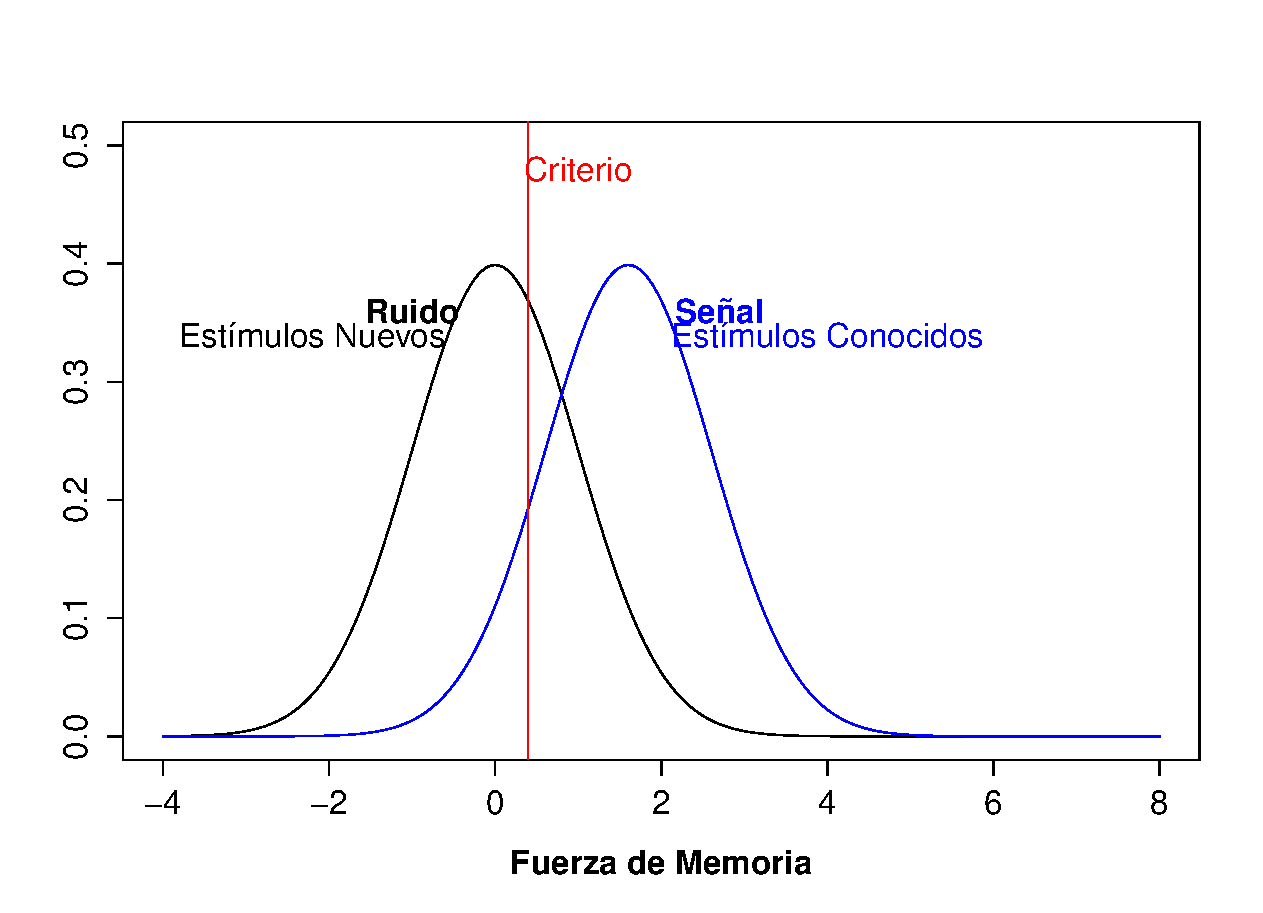
\includegraphics[width=0.60\textwidth]{Figures/RM_SDT_1} 
\decoRule
\caption[Variabilidad en la percepción de la señal]{Distribución normal representativa de cómo puede percibirse un estímulo concreto, asumiendo imprecisión en los sistemas sensoriales. El valor real del estímulo es el que más probablemente será percibido, (la media de la distribución, $\mu$) con cierto margen de error, (desviación estándar $\sigma$).}
\label{fig:Senal_percepcion}
\end{figure}

%Variabilidad en la presentación de la señal.
La misma idea aplica cuando hablamos de variabilidad en la presentación de la señal, sobretodo cuando esta consiste en una categoría o estado del mundo y no un estímulo concreto. Un ejemplo claro de ello son las pruebas clínicas. Por ejemplo, supongamos que un médico tiene que decidir si su paciente tiene una enfermedad particular con base en los resultados obtenidos en cierta prueba médica. La lectura de la evidencia arrojada por la prueba resulta un problema, en tanto que sabemos que las condiciones médicas suelen presentarse con una amplia variabilidad, por lo que tanto los síntomas reportados como los resultados obtenidos en una evaluación médica suelen variar entre persona y persona. Generalmente las pruebas médicas suelen indicar dentro de qué rango de valores puede encontrarse una persona con cierta condición, mismos que presuntamente se distribuyen normalmente al rededor de un valor típico, más probable de observar que el resto. La Figura ($HACER FIGURA$) captura esta idea, utilizando como ejemplo el rango de puntajes asociados con la ($condicion psicologica$) segun la prueba $Prueba$.\\


\begin{figure}[th]
\centering
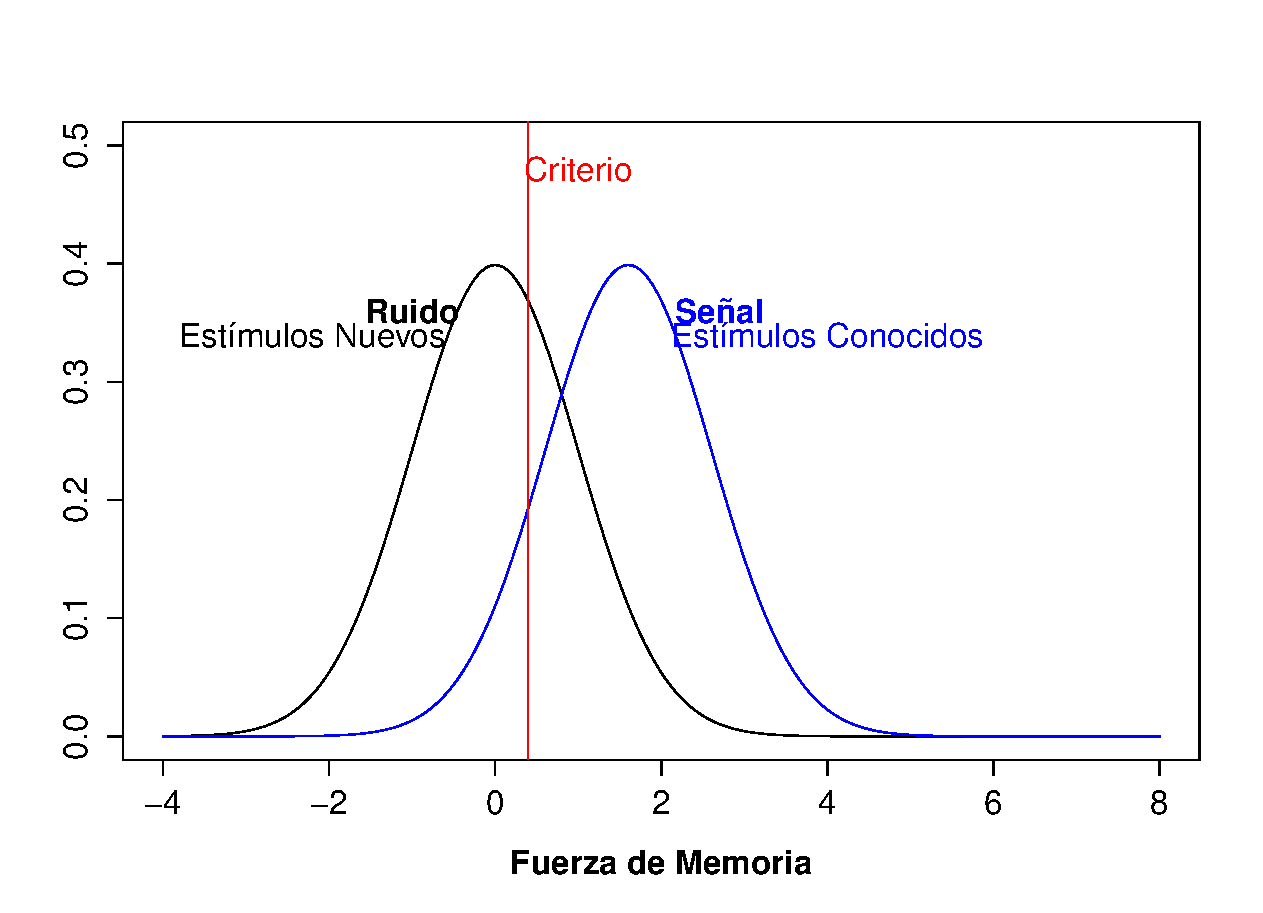
\includegraphics[width=0.60\textwidth]{Figures/RM_SDT_1} 
\decoRule
\caption[Variabilidad en la presentación de la señal]{Distribución normal que representa los puntajes en una prueba de depresión asociados con depresión. La figura captura la intuición de que existe un rango de valores que se asocian con la condición clínica con mayor o menor probabilidad, al rededor de un valor promedio.}
\label{fig:Senal_presentacion}
\end{figure}

      \item{Variabilidad en el Entorno: Ruido}

%La señal coexiste con el ruido y puede llegar a confundirse con el mismo.
Las señales, con toda su variabilidad, coexisten en el universo con otros estímulos.\\

algunos de los cuales pueden llegar a producir una evidencia similar a la de nuestra señal y ser, por tanto, confundidos con la misma. Esta idea se representa en la Figura 1 con la distribución normal negra identificada bajo el nombre de ruido, que se traslapa con cierta probabilidad con la distribución de señal.\\


El soporte de las distribuciones, identificado en la Figura 1 bajo el nombre de ‘Evidencia’ rara vez se define con precisión,  teniendo una concepción más bien abstracta; La idea general es que cuando queremos detectar una señal particular, comenzamos a recolectar un tipo de evidencia específico a la tarea ante la que nos encontramos. Lo más importante, es que la señal siempre va a estar asociada en mayor medida con dicha evidencia, distribuyéndose siempre en valores situados por encima (a la derecha, en la Figura 1) del ruido.\\


     \end{itemize}
 
  \item{El papel del Sesgo: La detección es decisión}

La TDS define toda tarea de detección como una tarea de decisión, donde el fin último por el cual el organismo se interesa en determinar si la señal está o no presente, es el de guiar su curso de acción. Es decir, el comportamiento de cualquier organismo va a depender de las señales que este detecta en su entorno.\\

Una consecuencia directa de la variabilidad involucrada en el entorno de decisión, es que el desempeño de todo sistema de detección es propenso a cometer errores y emitir un juicio de presencia o ausencia de la señal, que puede no coincidir con el estado del mundo. Dependiendo la correspondencia entre el estado del mundo y el juicio emitido por el sistema de detección, la TDS maneja las clasificaciones de respuesta mostradas en la Tabla 1; donde las celdas 2 y 3, corresponden a los errores posibles.\\

La TDS asume que el organismo fija un criterio de elección a lo largo del eje de la Evidencia, que va a determinar a partir de cuánta evidencia va a juzgar la señal como presente. Dicho criterio se va a representar como una línea transversal que atraviesa ambas distribuciones en una determinada altura, y se le va a identificar con el parámetro k. La TDS asume que los organismos van a fijar esta regla de elección, ponderando la información a la que tienen acceso con la información que poseen sobre la estructura de la tarea (i.e. cómo suele presentarse la señal, qué tan probable es que se presente, etc.)\\

    \begin{itemize}
      \item{Los errores cuestan y los aciertos pagan: Matrices de pago}\\

      \item{Sesgo o Preferencial}\\

  El sesgo se define como la preferencia del sistema a emitir respuestas de un tipo particular (i.e. 'Sí, detecto la señal' o 'No, no está'). La TDS cuenta con dos parámetros dedicados a la medición y evaluación del sesgo de los sistemas sometidos a tareas de detección.

 Sin embargo, no todos los errores tienen el mismo costo. Imaginemos el caso de una presa en potencia que busca determinar si el sonido que acaba de escuchar en la maleza corresponde o no con el de un depredador; no hay tiempo que perder, y el costo que dicho organismo tendría que pagar por cometer una falsa alarma (gasto innecesario de energía) o una omisión (morir devorado) es sustancialmente diferente. En este escenario particular, es muy probable que la presa sea mucho más propensa a correr por su vida, juzgando la presencia del depredador a partir de valores menores de evidencia.\\

Esta discrepancia en el peso que se le da a las consecuencias posibles de emitir una u otra respuesta y obtener uno de los cuatro posibles resultados, suele representarse en términos de una matriz de pagos, que nos ayude a definir cuáles son las consecuencias que el organismo buscará evitar o promover, según sea el caso, en mayor medida.\\

Ya sea por los distintos pesos que tengan las posibles consecuencias para el organismo, o porque se tiene una preferencia o predisposición inherente a decretar la presencia o ausencia de la señal, la TDS asume que el desempeño de los organismos que se enfrentan a tareas de detección de señales va a depender tanto de la calidad de la información a la que se tiene acceso (dentro de lo que se incluye la importancia de la variabilidad, que determina tanto la discriminabilidad de la señal como la sensibilidad del sistema ante la misma), como de un sesgo de elección.\\

La localización del criterio en nuestro eje de evidencia recolectada va a estar altamente influida por el sesgo que tenga nuestro sistema. Podemos hablar entonces de dos tipos distintos de sesgo: conservador y liberal. El primero, favorece la emisión de respuestas negativas al desplazar el criterio a la derecha y requerir al sistema la recolección de mayores niveles de evidencia antes de dar por detectada la señal. El segundo, promueve la detección de la señal, situando el criterio de elección hacia la izquierda, emitiendo un juicio de detección con valores menores de evidencia. Nótese que un sistema carente de sesgo, sería aquel que situara su criterio de elección justo en el punto en que las dos distribuciones se juntan, donde la probabilidad de cometer cualquiera de los tipos de acierto y errores, son iguales entre sí.\\

     \end{itemize}
\end{itemize}

\subsection{Parámetros del modelo}

Como se mencionó previamente, al realizar una tarea de detección existen dos posibles tipos de aciertos: al detectar la señal (Hits) y al rechazar el ruido (Rechazos), y dos posibles tipos de errores: los falsos positivos (Falsas alarmas) y los falsos negativos (Omisiones). La materia prima con base en la cual funciona el modelo propuesto por la TDS, son las tasas de aciertos y errores cometidos durante la tarea, de manera que por cada participante que pasa por una tarea de detección, tenemos cuatro tasas que describen su ejecución:

La Tabla 2 ilustra el cómputo de las cuatro tasas de ejecución, como una relación entre el resultado obtenido y el tipo de ensayo con base en el que se le definió como tal. Es decir, tenemos dos tasas definidas en relación al número total de ensayos con la señal (la tasa de hits y la tasa de omisiones) que nos dicen qué proporción de los ensayos con señal fueron detectados correctamente y cuáles se dejaron pasar; y tenemos dos tasas definidas en relación al total de ensayos con ruido (la tasa de falsas alarmas y la tasa de rechazos correctos) que nos describen la relación de los ensayos con ruido que fueron discriminados correctamente y aquellos que se confundieron con la señal.

Para realizar el análisis de datos, bajo el marco de la TDS, sólo necesitaremos un par de estas tasas: la tasa de hits y la tasa de falsas alarmas. Esto bajo el entendido de que las tasas de omisión y rechazos correctos no son más que su complemento, respectivamente, y que estas dos tasas contienen toda la información que necesitamos sobre el desempeño de los participantes.

La idea general de la importancia de estas tasas de ejecución, es que cada una representa el área de las distribuciones de ruido y señal que cae a la izquierda o derecha del criterio de decisión.

Para la estimación paramétrica se utiliza la misma lógica, pero se sigue el procedimiento inverso. Dado que no podemos observar ni cuantificar de manera directa el criterio usado por los participantes para responder a la tarea, qué tan juntas o separadas se encuentran las distribuciones de ruido y señal para cada participante o qué tipo de sesgo pudieran estar siguiendo, utilizamos las tasas de ejecución para hacer inferencias sobre la localización del criterio, la diferencia entre las medias de ambas distribuciones y el grado en que una respuesta se favorece sobre otra. 

A partir de ahora comenzaremos a hablar sobre cómo se calculan cada uno de los parámetros del modelo, de acuerdo a la teoría clásica que sigue los supuestos estadísticos previamente descritos.  Es importante aclarar que el Graficador de Tasas previamente expuesto no representa la teoría con entera precisión; el propósito de ese primer Graficador es simplemente ilustrar cómo describe la TDS el comportamiento de un sistema que se enfrenta ante una tarea de detección, donde existen dos distribuciones que se sobreponen. El Graficador permite manipular directamente la localización del criterio, con la simpleza que implicaría desplazar una línea vertical sobre el eje de decisión y ver qué consecuencias tiene sobre la probabilidad de obtener un tipo particular de acierto o error.


Antes de ahondar a detalle en los parámetros, hay que declarar un par de supuestos formales que hace la Teoría para facilitar la representación gráfica del modelo y la estimación paramétrica:

\begin{enumerate}
\item En su forma clásica, la TDS asume que las distribuciones de ruido y señal son distribuciones normales.
  \begin{itemize}
  \item 
  \end{itemize}
\item En su forma estándar, se asume que las distribuciones de ruido y señal son equivariantes, (compartiendo una desviación estándar de 1).
  \begin{itemize}
  \item 
  \end{itemize}
\item La distribución de ruido tiene su media en 0. 
  \begin{itemize}
  \item La estimación de todos los parámetros del modelo de detección de señales se hace tomando como referencia la distribución del ruido (con  media 0 y desviación estándar de 1)
  \end{itemize}
\end{enumerate}



\begin{itemize}
\item Discriminabilidad $(d')$

La discriminabilidad se representa en los modelos de detección de señales con un parámetro $d'$, que representa la distancia entre las medias de las distribuciones de ruido y señal. 

Para encontrar la distancia entre las medias de la distribución de ruido y señal, necesitamos saber el punto en que el criterio toca cada distribución. Para ello, calculamos las probabilidades complementarias a las tasas de hits y falsas alarmas y las traducimos a puntajes Z (Ver Fig. 3). Dado que el puntaje Z funciona como una medida de dispersión de la media, basta con restar el puntaje Z de la intersección del criterio con la distribución de señal a el puntaje Z de intersección con la distribución de ruido para conocer la localización de la media de la señal. Por definición, d’ sólo puede tener valores positivos ya que la teoría asume que la distribución de señal siempre está a la derecha de la distribución de ruido porque contiene una mayor cantidad de la evidencia con base en la cual se hace el juicio de detección de la señal.



\item Criterio  $k$

Una vez que hemos resumido el desempeño de nuestro participante en la tarea de detección, el parámetro cuya estimación resulta más sencilla y directa es el Criterio (k). Entender cómo se computa el parámetro nos requiere únicamente de mantener presente el supuesto de que el Ruido se distribuye normalmente y se va a localizar siempre a la izquierda de la señal, por lo que le asignamos una media de cero para tener un punto de referencia para estimar el espacio en que se desarrollan el resto de los parámetros. \\

Para calcular el criterio lo único que necesitamos es conocer la tasa de Falsas Alarmas, que tal y como mencionábamos en el segmento anterior, nos indica qué proporción de la distribución de ruido cae a la derecha del criterio. Dado que a la distribución de ruido, le fue asignada arbitrariamente una media de cero, podemos asignar un valor al punto en que el criterio corta la distribución de ruido y define las tasas de Rechazos y Falsas Alarmas obtenidas por el participante. Conociendo el área de la distribución de Ruido que cae bajo el criterio, (el complemento de la tasa de Falsas Alarmas, o bien, la Tasa de Rechazos correctos), y sabiendo que la distribución tiene una desviación estándar de 1, podemos convertir el valor de la tasa (que corresponde a la probabilidad de cometer un rechazo correcto, de acuerdo al área bajo la curva) en Puntajes Z y conocer la localización del criterio.\\

 El parámetro k, por lo general, va estar representado por un número natural (un número positivo), que indica en términos de Puntajes Z  la posición del criterio sobre el eje de decisión, relativo a la distribución de ruido con media cero. El criterio sólo tiene valores positivos, porque normalmente se espera que la tasa de falsas alarmas nunca tenga un valor mayor a 0.5 (las consecuencias de una tasa de Falsas Alarmas tan alta, se expondrán con más claridad en el apartado correspondiente a la d’. \\


\item Sesgo - $\beta$

El parámetro más comúnmente utilizado en la literatura para evaluar el sesgo de los participantes en estudios donde se aplica el modelo de detección de señales al análisis de tareas experimentales, es Beta ($\beta$). Se define como una razón entre la probabilidad con que la evidencia  \\

$\beta = \frac{p(Signal)}{p(Noise)}$

si $\beta<1$ o C<0, sabemos se trata de un sesgo liberal y si $\beta>1$, C>0, hablamos de un sesgo conservador.\\

\item Sesgo - $C$


\end{itemize}   %Terminan los parametros



%----------------------------------------------------------------

\subsection{Tareas de detección}

\begin{itemize}
\item Tareas de detección binaria 

En el laboratorio, la  TDS se estudia a partir  de tareas de detección donde se expone a un  sujeto  a  N  número  de  ensayos,  (comprendidos  por  n  ensayos con  sólo  ruido  y  n  ensayos donde  el  ruido  viene  acompañado  de  la  señal)  ante  los  que  se  le  pide  al  participante  que responda eligiendo una de dos opciones: Sí está la señal o No está la señal. En estos escenarios controlados,  el  experimentador  decide  la  proporción  de  ensayos  con  y  sin  señal  que  se presentarán, así como la matriz de pagos que definirán la utilidad de sus aciertos y errores. \\


\item Tareas con escala de confianza

Un segundo procedimiento comúnmente utilizado en tareas de detección implica añadir un paso adicional a la tarea de los participantes. 


\item Tarea con elección forzada entre dos alternativas.
\end{itemize}

